\documentclass[a4paper,11pt,reqno]{amsart}

% --------------------------------------------------------
% Packages
% --------------------------------------------------------
\usepackage[utf8]{inputenc}
\usepackage[foot]{amsaddr}
\usepackage{amsmath,amsfonts,amssymb,amsthm,mathrsfs,bm}
\usepackage[margin=0.95in]{geometry}
\usepackage{color}
\usepackage[dvipsnames]{xcolor}
\usepackage{mathtools,graphicx}
\usepackage{tcolorbox}
\usepackage{listings}
\usepackage{textcomp}
\usepackage{hyperref}

% --------------------------------------------------------
% Custom Colours
% --------------------------------------------------------
\definecolor{CommentGreen}{rgb}{0.0,0.4,0.0}
\definecolor{Background}{rgb}{0.9,1.0,0.85}
\definecolor{lrow}{rgb}{0.914,0.918,0.922}
\definecolor{drow}{rgb}{0.725,0.745,0.769}


% --------------------------------------------------------
% Typesetting Python code
% --------------------------------------------------------
\lstloadlanguages{Python}%
\lstset{
    language=Python, upquote=true, frame=single,
    basicstyle=\small\ttfamily,
    backgroundcolor=\color{yellow!30},
    keywordstyle=[1]\color{NavyBlue}\bfseries,
    keywordstyle=[2]\color{RubineRed},
    keywordstyle=[3]\color{orange!90}\bfseries,
    keywordstyle=[4]\color{Green!90}\bfseries,
    identifierstyle=,
    commentstyle=\usefont{T1}{pcr}{m}{sl}\color{MidnightBlue}\small,
    stringstyle=\color{purple},
    showstringspaces=false, tabsize=4, morekeywords={import,as},
    morekeywords=[2]{args,__init__},
    morekeywords=[3]{@property},
    morekeywords=[4]{self},
    morecomment=[l][\color{blue}]{...},
    numbers=none, firstnumber=1,
    numberstyle=\tiny\color{blue},
    stepnumber=1, xleftmargin=10pt, xrightmargin=10pt
}

\synctex=1

\hypersetup{
    unicode=false, pdftoolbar=true, 
    pdfmenubar=true, pdffitwindow=false, pdfstartview={FitH}, 
    pdftitle={ELE2024 Coursework}, pdfauthor={A. Author},
    pdfsubject={ELE2024 coursework}, pdfcreator={A. Author},
    pdfproducer={ELE2024}, pdfnewwindow=true,
    colorlinks=true, linkcolor=red,
    citecolor=blue, filecolor=magenta, urlcolor=cyan
}

% --------------------------------------------------------
% CUSTOM COMMANDS
% --------------------------------------------------------
\renewcommand{\Re}{\mathbf{re}}
\renewcommand{\Im}{\mathbf{im}}
\newcommand{\R}{\mathbb{R}}
\newcommand{\N}{\mathbb{N}}
\newcommand{\C}{\mathbb{C}}
\newcommand{\lap}{\mathscr{L}}
\newcommand{\dd}{\mathrm{d}}
\newcommand{\smallmat}[1]{\left[ \begin{smallmatrix}#1 \end{smallmatrix} \right]}

% --------------------------------------------------------
% Opening: Title and Author Names
%          Modify this section
% --------------------------------------------------------
\title[ELE2024 Coursework]{Report for the ELE2024 coursework}

\author[B. Harkin]{Ben Harkin}
\author[D. Lim]{David Lim}
\author[C. Watts]{Cerys Watts}
\address[B. Harkin, D. Lim and C. Watts]{Email addresses: \href{mailto:bharkin02@qub.ac.uk} {bharkin02@qub.ac.uk}, \href{mailto:dlim04@qub.ac.uk}{dlim04@qub.ac.uk} and \href{mailto:cwatts06@qub.ac.uk}{cwatts06@qub.ac.uk}.}
\thanks{Some note goes here.  Version 0.0.1. Last updated:~\today.}



% --------------------------------------------------------
% Beginning of your document
% --------------------------------------------------------
\begin{document}

\maketitle


\section{Part A: Control Theory}
    \subsection{Given Equations} The following equations were given by Dr P. Soposakis as part of the coursework brief:

\begin{equation} \label{eq:1}
    L = L_0 + L_1 exp(-\alpha y)
\end{equation}

\begin{equation} \label{eq:2}
    F_{mag}=c \frac{I^2}{y^2}
\end{equation}

    \subsection*{Problem A1}\label{sec:q1} Use first principles from physics, as well as Equations \eqref{eq:1} and \eqref{eq:2}, to derive a system of ordinary differential equations that describes how the input voltage, \(V\) , affects the position, \(x\), of the ball on the inclined plane. Note: introduce an inertial frame of reference where counterclockwise rotations are positive.
    
    \begin{align}
        F_{spring} &= k(x - d)\\
        F_{damper} &= b\dot{x}\\
        F_{mag} &= c \frac{I^2}{y^2} \text{, where } y = d - x
    \end{align}

    \begin{align}
        -Tr &= I\ddot{\theta}\\
        a &= \ddot{x} = \ddot{\theta r}\\
        \therefore T &= \frac{I \ddot{\theta}}{r}\\
        \ddot{\theta} &= \frac{\ddot{x}}{r}\\
        I &= \frac{2}{5} mr^2
    \end{align}
    
    \begin{align}
        T &= - \frac{2mr^2 \ddot{x}}{5r^2} \nonumber \\
        T &= - \frac{2m \ddot{x}}{5}
    \end{align}
    
    \begin{align}
        F &= m \ddot{x} \nonumber \\
        F_{mag} + mg \sin{\phi} - T - F_{spring} - F_{damper} &= m \ddot{x} \nonumber \\
        \frac{cI^2}{y^2} + mg \sin{\phi} + \frac{2m \ddot{x}}{5} - k(x - d) - b \dot{x} &= m \ddot{x}
    \end{align}
    
    \begin{align}
        V_{R} &= IR\\
        V_{L} &= L \dot{I}\\
        L &= L_{0} + L{1} \exp(- \alpha y) \text{, where } y = d - x
    \end{align}
    
    \begin{align}
        V &= V_{R} + V_{L} \nonumber \\
        V &= IR + L \dot{I} \nonumber \\
        V &= IR + (L_{0} + L_{1} \exp(- \alpha y)) \dot{I} \nonumber \\
        \nonumber \\
        V &= IR + (L_{0} + L_{1} \exp(- \alpha (d - x))\dot{I}
    \end{align}
    
    \begin{align}
        \frac{cI^2}{y^2} + mg \sin{\phi} + \frac{2m \ddot{x}}{5} - k(x - d) - b \dot{x} &= m \ddot{x} \nonumber \\
        \frac{cI^2}{y^2} + mg \sin{\phi} - k(x -d) - b \dot{x} &= m \ddot{x} - \frac{2m \ddot{x}}{5} \nonumber \\
        \frac{cI^2}{y^2} + mg \sin{\phi} - k(x -d) - b \dot{x} &= \frac{3m}{5} \ddot{x} \nonumber \\
        \nonumber \\
        \frac{cI^2}{(d - x)^2} + mg \sin{\phi} - k(x -d) - b \dot{x} &= \frac{3m}{5} \ddot{x}
    \end{align}
    
    \subsection{Problem A2}
    Refer to other sections as Section~\ref{sec:q1}. An example of a numbered list
    \begin{enumerate}
        \item first item,
        \item second item.
    \end{enumerate}
    Links are \href{https://google.com}{like this}. We also have \textbf{boldface}, \textit{italics},
    \emph{emphasised}, \texttt{truetype}, \textsc{Small Caps} and so on.

    \subsection*{Problem A3} 
\hfill \break
According to Proposition 3.4 in the textbook, the equilibrium points of Equation \eqref{eq:16} are:
\hfill \break
\begin{equation}
(x_1^e, x_2^e, I^e) = 
    \begin{cases}
        \hspace{3cm}x_2^e = 0\\    
        \frac{5cI^e^2}{3m(\delta - x_1^e)^2} + \frac{5g\sin{\phi}}{3} - \frac{5k}{3m}(x_1^e -d) &= 0   
    \end{cases}
\end{equation}
\hfill \break
According to Proposition 3.4 in the textbook, the equilibrium points of Equation \eqref{eq:17} are:
\hfill \break
\begin{equation}
(I^e, V^e) = 
    \begin{cases}
        \frac{V^e - {I_1^e}R}{\left(L_{0} + L_{1} ^{- \alpha (d - x)}\right)} = 0
    \end{cases}
\end{equation}
    \subsection*{Problem A4} Linearise the system at an equilibrium point (use deviation variables).
    \begin{align}
        {\dot{x_2}} &= {\frac{CI^2}{(d -{x_1^\text{eq}})^2}}+{\frac{5}{3}g\sin{\phi}}-{\frac{5k}{3m}{(x_1 - d)}}-{\frac{5b}{3m}{x_2}}\nonumber
    \end{align}
    \begin{align}
        {\dot{x_2}} &= {\frac{5c}{3m}( \frac{I^2}{(d -{x_1})^2} -  \frac{I^{\text{eq}2}}{(d -{x_1^\text{eq}})^2})}-{\frac{5k}{3m}{(x_1 -
        {x_1^\text{eq}})}}-{\frac{5b}{3m}{x_2}}\nonumber
    \end{align}
    \begin{align}
        {\dot{x_2}} &= {\frac{5c}{3m}( \frac{2I^2}{(d -{x_1})^2}(I - I^\text{eq}) -  \frac{2I^{\text{eq}2}}{(d -{x_1^\text{eq}})^3}(x_1 - {x_1^\text{eq}}))}-{\frac{5k}{3m}{(x_1 -
        {x_1^\text{eq}})}}-{\frac{5b}{3m}{x_2}}\nonumber
    \end{align}
    \begin{align} 
        \nonumber 
        \bar{I} &= I - I^\text{eq} \\ \nonumber 
        \bar{x_1} &= {x_1} - {x_1^\text{eq}} \\ \nonumber
        \bar{x} &= {x_2} - {x_2^\text{eq}} \\ \nonumber &= {x_2} \\ \nonumber
    \end{align}
    \begin{align}
        {\dot{x_2}} &= {\frac{5c}{3m}( \frac{2I^\text{eq}}{(d -{x_1})^2}\bar{I} -  \frac{2I^{\text{eq}2}}{(d -{x_1^\text{eq}})^3}\bar{x_1})}-{\frac{5k}{3m}{\bar{x_1}}}-{\frac{5b}{3m}\bar{x_2}}\nonumber
    \end{align}

    \subsection*{Problem A5}Determine the transfer function of the linearised system that you determined in Problem A4. The input of the system is the voltage across the circuit and the output is the position of the ball on the inclined plane. How many poles does this transfer function have? Derive sufficient conditions on the system parameters under which the impulse response of the transfer function is oscillatory.

    
\section{Part B: Analysis and Controller Design}
    \subsection*{Problem B1}
\hfill \break
The wooden ball is limited to where it can equilibrate  by the physical limits of the system.\\
$x_{max}$ is the point furthest down the slope where the ball can equilibrate. This cannot be any further down the slope than the location of the electromagnet. This location is denoted on Figure \ref{fig:system} with $\delta$.\\
$\therefore$ We can say that $x_{max}$ can be no greater than $\delta$.\\
The limit of where the ball could equilibriate on the upper end of the slope is denoted by $x_{min}$. $d$ is the natural length of the spring, so $x_{min}$ can be no less than that, but we also need to take into account the downward force of the ball. This downward force is denoted in Figure \ref{fig:system} with $mg\sin{\phi}$. \\
However, the ball is not free to roll unobstructed. Taking into account the stiffness of the spring $k$, we can see that $x_{min}$ can be no smaller than $d + \frac{mg\sin{\phi}}{k}$.\\
$\therefore$ We can say that the system can only equilibrate at those positions $x^e$ that satisfy: \\
\begin{equation}
    d + \frac{mg\sin{\phi}}{k} < x^e < \delta
\end{equation}
To calculate the equilibrium voltage and current we use Equation \eqref{eq:10}. 
\begin{equation} \nonumber
    \frac{cI^2}{(\delta - x)^2} + mg \sin{\phi} - k(x -d) - b \dot{x} &= \frac{3m}{5} \ddot{x}
\end{equation}
To equilibriate, velocity and acceleration are equal to zero: \\
\begin{align} 
    \therefore \frac{cI^2}{(\delta - x)^2} + mg \sin{\phi} - k(x -d)  = 0 \nonumber \\
    \frac{-cI^2}{(\delta - x)^2} = mg \sin{\phi} - k(x -d) \nonumber \\
    \therefore I^e = \sqrt{\frac{(mg\sin{\phi}) - k(x_1^e - d)}{-c}(\delta - x_1^e)^2}
\end{align}
\begin{align} 
    V^e &= I^e \cdot R \nonumber \\
    \therefore V^e &= \left(\sqrt{\frac{(mg\sin{\phi}) - k(x_1^e - d)}{-c}(\delta - x_1^e)^2} \right) R
\end{align}
    \subsection*{Problem B2}

    The linearisation of the system was tested by writing simulating both systems in Python. The implementation of the simulations can be found \href{https://github.com/drlim2u/ELE2024-Control-Coursework/blob/4dc7e6f918fce68ee3aef799fe1dba15ea789481/PartB.py#L44}{here}.

    \begin{figure}[H]
        \centering
        \includegraphics[width=0.6\linewidth]{figures/problem_b2_a.eps}
        \caption{Three plots of the simulation of the non-linear system with the \(x\) position, \(\dot{x}\) and \(I\) of the ball in respect to time.}
        \label{fig:problem_b2_a}
    \end{figure}
    
    \begin{figure}[H]
        \centering
        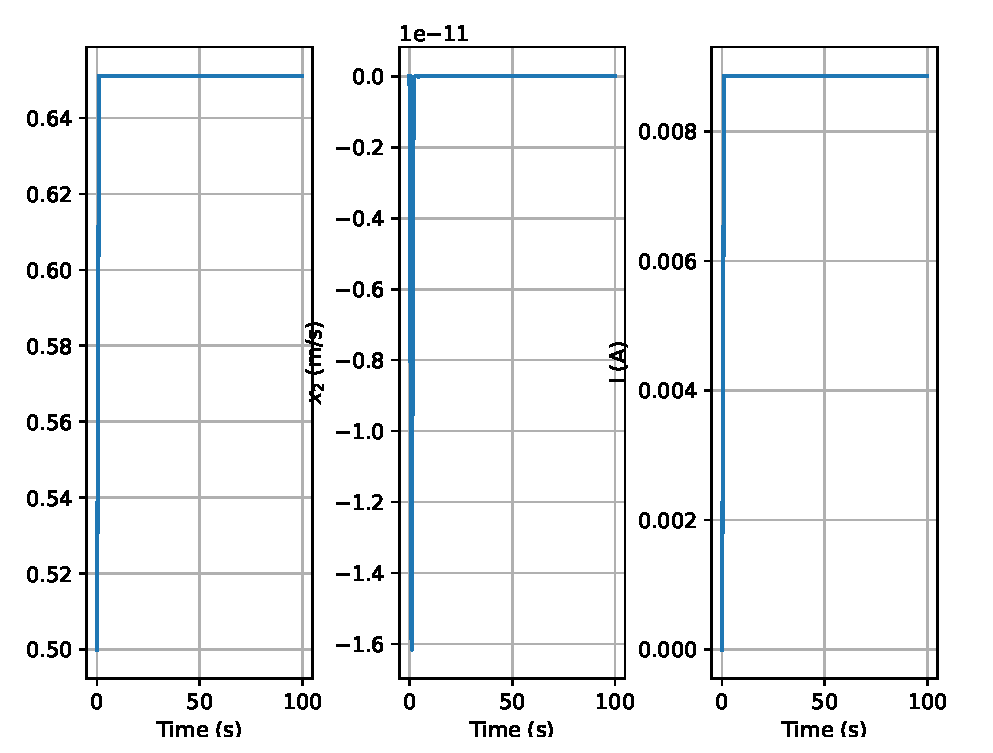
\includegraphics[width=0.6\linewidth]{figures/problem_b2_b.eps}
        \caption{Three plots of the simulation of the linearised system with the \(x\) position, \(\dot{x}\) and \(I\) of the ball in respect to time.}
        \label{fig:problem_b2_b}
    \end{figure}
    
    As can be seen in both Figure \ref{fig:problem_b2_a} and Figure \ref{fig:problem_b2_b} both simulations showed stable systems. However the non-linear system shown in Figure \ref{fig:problem_b2_a} does not behave close to the equilibrium point of the linearised system shown in Figure \ref{fig:problem_b2_b}. The non-linear system shows an equilibrium point of \(x_1\) at around 0.42m whereas the linearised system shows that the equilibrium point of \(x_1\) is around 0.65m. It can therefore be determined, assuming that the simulation was programmed correctly, that there is an error in the linearisation. It is believed that this issue comes specifically from the linearisation of \(\dot{I}\).

    \subsection*{Problem B3}
    A simulation was run to determine the impulse response and the step response of the transfer of the linearised system. This simulation was written in Python for which the code can be found \href{https://github.com/drlim2u/ELE2024-Control-Coursework/blob/059953dc7b2d8ba0a86b6f437153ceb4442b7a60/PartB.py#L59}{here} and which produced the Figure \ref{fig:problem_b3} below.
    \begin{figure}[H]
        \centering
        \includegraphics[width=0.6\linewidth]{figures/problem_b3.eps}
        \caption{Graph showing both impulse response and step response of the transfer function of the linearised system.}
        \label{fig:problem_b3}
    \end{figure}

  
    \subsection*{Problem B4}
    \hfill \break
    A simulation was run to determine the low-frequency and high-frequency asymptotes of the magnitude and phase lag of the transfer function of the linearised system. This simulation was written in Python for which the code can be found \href{https://github.com/drlim2u/ELE2024-Control-Coursework/blob/059953dc7b2d8ba0a86b6f437153ceb4442b7a60/PartB.py#L125}{here} and which produced the Figure \ref{fig:problem_b4} below.
    \begin{figure}[H]
        \centering
        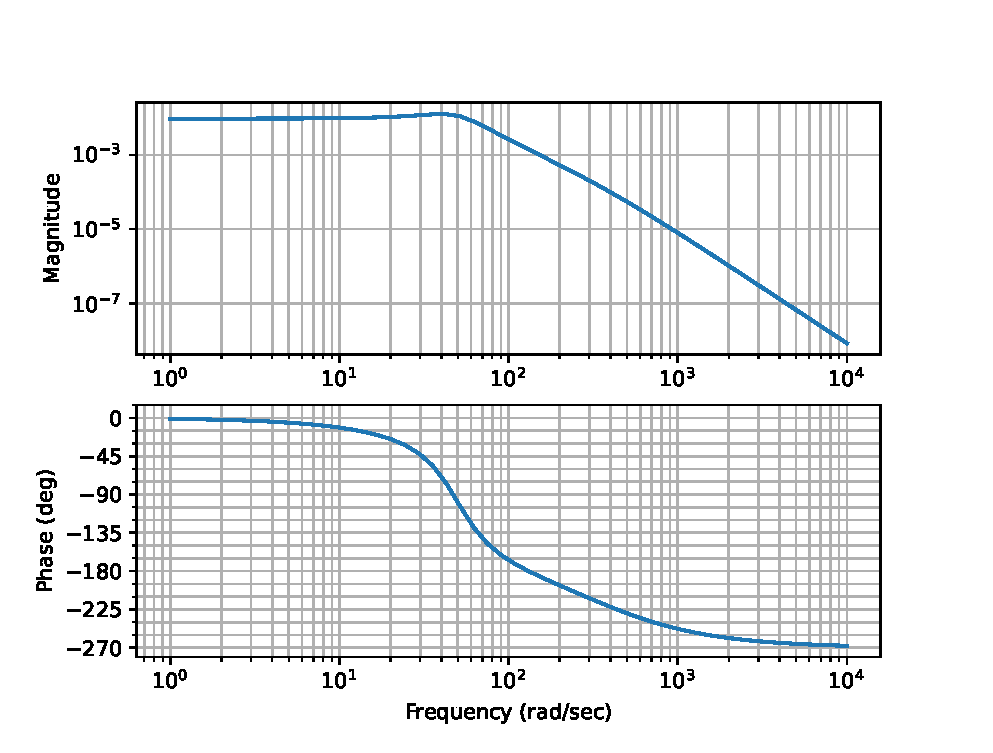
\includegraphics[width=0.6\linewidth]{figures/problem_b4.eps}
        \caption{Graphs showing both low-frequency and high-frequency asymptotes of the magnitude and phase lag of the transfer function of the linearised system.}
        \label{fig:problem_b4}
    \end{figure}
    \subsection*{Problem B5}
\hfill \break 
The desired characteristics of a controller: \\
BIBO stability is a critical benchmark for our system to reach. To be exact, bounded changes in the set point should only cause bounded changes in the output \\
We should want the system to converge on a point quickly but with as little oscillation as possible. To do this the system would need to penalise large lateral velocities in the system. It would be preferable for the ball to move slower and reach the point with low oscillation than for it to come in contact with the physical boundaries of the system.\\
Evidence it is a good controller:\\
As George Box once said: "All models are wrong". What we aim for in a model may not be seen in practise. The evidence we would have to show it is a good controller would be a very similar measurement from our laser proximity sensor as what our model would estimate. The \emph{offset} should be as low as possible. The model also has to take into account the physical boundaries of the system that we explore in Problem B1. 
    \subsection*{Problem B6}
    \hfill \break
    To control the system a Proportional Integral Differential (PID) controller was designed. The integral part of the PID controller will adjust for physical boundaries of the system and account for systematic errors and hopefully reduce and remove offset. This helps achieve the desired characteristic set out in Problem B5. The controller was written in Python and the implementaion can be found \href{https://github.com/drlim2u/ELE2024-Control-Coursework/blob/059953dc7b2d8ba0a86b6f437153ceb4442b7a60/PartB.py#L187}{here}. The step response from the simulated controlled system was recorded and is shown below in Figure \ref{fig:problem_b6}.
    
    \begin{figure}[H]
        \centering
        \includegraphics[width=0.6\linewidth]{figures/problem_b6.eps}
        \caption{Graph to show the step response of the system with a PID controller implemented.}
        \label{fig:problem_b6}
    \end{figure}
    
    As Figure \ref{fig:problem_b6} shows the system's impulse response settles very quickly.

    
\section{Part C: Bonus Questions}
    \subsection{Problem C1} Determine the Laplace transform of f(t) = \(\log{\left(t^{3} \right)}\), \(t > 0\).

    \medskip
    The solution is:
    
    \smallskip
     \begin{equation}
         \left( \frac{\sqrt{3} \left(- {G_{5, 2}^{2, 3}\left(\begin{matrix} \frac{2}{3}, \frac{1}{3}, 0 & 1, 1 \\0, 0 &  \end{matrix} \middle| {\frac{27}{s^{3}}} \right)} + {G_{5, 2}^{0, 5}\left(\begin{matrix} \frac{2}{3}, \frac{1}{3}, 0, 1, 1 &  \\ & 0, 0 \end{matrix} \middle| {\frac{27}{s^{3}}} \right)}\right)}{2 \pi s}, \  0, \  \text{True}\right)
     \end{equation}
 
    \subsection{Problem C2} Determine the Laplace transform of f(t) = \(\left|{\cos{\left(w \right)}}\right|)\), \(t \geq 0\), \(w > 0\).

    \medskip
    The solution is:

    \smallskip
     \(\left( \frac{\left|{\cos{\left(\omega \right)}}\right|}{\omega}, \  0, \  \text{True}\right)\)

    \input{Report/Part C/Problem C3}

\section{Part D: Planning, Organisation \& Collaboration}
    \subsection*{D1}
    We used a GitHub repository to collaborate on writing code. We used the git issue tracker to keep track of the tasks. This issue tracker was critical as it allowed us to see how the tasks were assigned and how those tasks were progressing. We distributed the tasks on an initial call where we took problems that we felt confident with. These changed as we went on and might have found some problems tougher than we expected. Regular communication was the key to ensuring we were all aware of the progress on projects. The link to the issue tracker can be found  \href{https://github.com/drlim2u/ELE2024-Control-Coursework/issues}{here}.
    \subsection{D2}
    \begin{enumerate}
        \item We communicated clearly
        \item We began early and kept on top of our work.
        \item We all taught each other new things. etc
    \end{enumerate}
    \subsection*{D3}
    \hfill \break
    The current global situation was a massive challenge to the group. Not only did it effect how the group met and communicated in which was the first group project started during the pandemic for all of us, but this period has also been a significant struggle and has effected academic performance for some of the members in the group.\\
    
    The fact that we were physically apart meant communication was limited to calls, texts and emails. Because these forms of communication are inherently more limited than face-to-face conversing it was important that we we communicate, we clearly define the goals of it. Things like the issue tracker in GitHub was key to ensuring we were all on the same page when it came to progress and outstanding tasks. In hindsight weekly voice or video meetings should've been implemented as although the group had constant contact through social media it was difficult to stay motivated for some members in the group especially in the aforementioned global situation.\\
    
    The coursework assignment was structured more linearly than expected which didn't inherently enable a simultaneous workflow. This meant that even though we started earlier than most groups we were still pushed for time as we found that tasks had to be completed in a set order and the way tasks were distributed in the beginning meant that group members were sometimes left waiting for someone to finish a task. This could've been helped by encouraging more people to engage with every task rather than splitting tasks up as you would in a traditional workload.\\
    
    Finally, towards the submission dealing David started showing symptoms of COVID-19. Thankfully he tested negative in the following days however this was added stress to an already stressful situation and coursework due to the amount of work needed to complete it. However, Ben and Cerys managed to rise up to the challenge and get a version of this coursework submitted in time in case David's exceptional circumstances form was rejected.


\end{document}
